\documentclass{article}

\usepackage{amsmath,amssymb}
\usepackage{geometry}
\usepackage{graphicx}

\geometry{a4paper, margin=2.5cm}

\begin{document}

% ============================================================
\section*{Offline Reinforcement Learning: CQL and IQL}

\subsection*{First, a story}

A coach receives an unusual assignment: the team has disbanded and he can no longer hold training sessions --- all he has is an archive of last season's match recordings. The recordings capture every decision in every situation and its outcome. From this archive alone he must write next season's tactical manual.

\textbf{Naive RL's approach}: treat the recordings as a free training ground --- replay them over and over until the Q function and policy ``practice'' to convergence.

\textbf{The surprising outcome}: the drilled manual works fine on situations covered by the recordings, but whenever a situation arises that the recordings never showed, the coach's instructions turn absurd --- the overall level ends up \emph{below} simply copying the recordings verbatim (behavior cloning).

\textbf{The core question of this chapter}: with only a fixed dataset and no further interaction, how do we learn a policy that does not collapse?

\[
\boxed{\text{Access only a fixed dataset } \mathcal{D}=\{(s,a,r,s',d)\},\quad \text{learn } \pi \text{ maximizing } \mathbb{E}_\pi\!\Big[\sum_t \gamma^t r_t\Big]}
\]

The disease is called \textbf{distribution shift}: the offline-learned policy probes state--action pairs the dataset barely covers, where the network's answers are pure hallucination, and bootstrapping amplifies the errors.

The good news: the field has two equally mature ``prescriptions'' with opposite philosophies:

\textbf{CQL (prescription 1)}: even if unseen actions must be evaluated, \textbf{push their value estimates down} --- write pessimism into the value function.

\textbf{IQL (prescription 2)}: \textbf{never evaluate unseen actions at all} --- pick high-value actions only within the data's support, writing pessimism into the action set.

\subsection*{Formalization}

\textbf{The offline dataset}: $\mathcal{D}$ is generated by some \textbf{behavior policy} $\mu$; its coverage is determined by $\mu$'s occupancy $d^\mu(s,a)$. The data is one-shot --- $\mathcal{D}$ cannot grow.

\begin{itemize}
  \item $\mathcal{D}$ --- the fixed dataset, read-only during training;
  \item $\mu$ --- the behavior policy, the dataset's ``origin'', which we cannot access or use for further interaction;
  \item $d^\mu(s,a)$ --- the behavior policy's occupancy; the data covers only its support;
  \item $a\sim\pi(\cdot|s)$ vs.\ $a\sim\mu(\cdot|s)$ --- the mismatch between learned policy and data distribution, the source of distribution shift.
\end{itemize}

\textbf{In plain words}: in online RL the policy can query the environment at every step and correct mistakes immediately; in offline RL there is no such query --- once the network asks a question outside the data, nobody checks whether the answer is true.

% ============================================================
\section*{Extrapolation Error: why naive offline Q-learning collapses}

\subsection*{$\max$ is the culprit}

Recall DQN's target:
\[
y = r + \gamma \max_{a'} Q_{\bar\theta}(s', a')
\]

Online, continued interaction keeps calibrating the overestimations that $\max$ selects; offline, $\max$ ranges over the network's estimates of \textbf{all actions} (including ones never present in the dataset), and no new data ever corrects them. For unseen actions $Q_{\bar\theta}(s',a')$ has never been calibrated by any target --- its value is the network's ``free improvisation'' --- and $\max$ reliably picks the ``relatively highest'' one, which is precisely the out-of-data, untrustworthy one. That untrustworthy high value then feeds back as a bootstrap target and amplifies: Q estimates \textbf{decouple} from true values, the greedy policy acts on them, and real returns collapse (Figure~1).

Fujimoto et al.\ named the dominant source --- actions absent from the data --- \textbf{extrapolation error}; the survey of Levine et al.\ (2020) decomposes this error class into three sources:

\begin{itemize}
  \item \textbf{Actions absent from the data}: the $a'$ selected by $\max$ never appears in $\mathcal{D}$; Q has no basis for it;
  \item \textbf{State mismatch}: $s'$ is rare (or absent) in $\mathcal{D}$, making all of that state's action estimates untrustworthy;
  \item \textbf{Dynamics mismatch}: even if $(s',a')$ is in the data, the assumed offline transition may differ from the true environment.
\end{itemize}

\begin{figure}[!htbp]
  \centering
  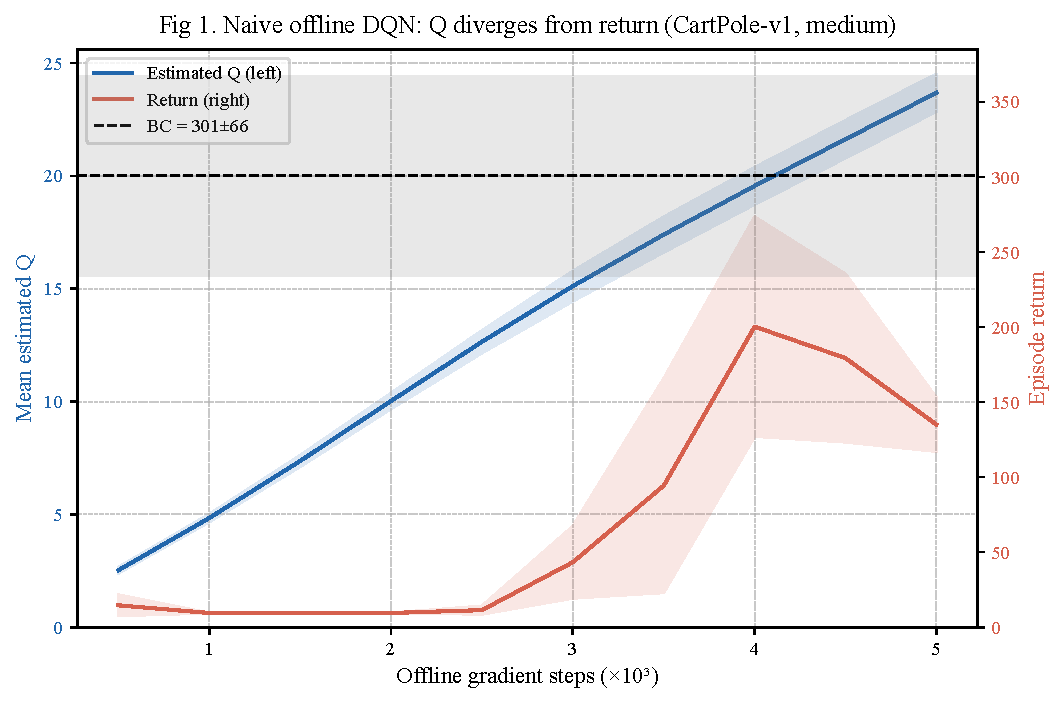
\includegraphics[width=0.88\textwidth]{fig1_ood_overestimation.pdf}
  \caption{The extrapolation-error collapse of naive offline DQN (CartPole-v1, medium dataset, 3 random seeds, shading $\pm 1\sigma$). In one plot: the blue curve (left axis) is the Q network's max-Q estimate on data states --- it no longer tracks the policy's true value; the red curve (right axis) is the greedy policy's true return, improving briefly then falling, and staying far below the behavior-cloning (BC) ``pass line'' (BC is about 300; see the gray band in Figure~2). The decoupling of Q estimates from true returns is exactly what extrapolation error entering the bootstrap targets looks like.}
  \label{fig:offline-overestimation}
\end{figure}

\subsection*{Q decoupling from true value}

Overestimation is not simply ``large Q numbers''. Diagnosing an offline algorithm means checking whether \textbf{Q estimates and true returns track each other}: in Figure~1 the naive offline DQN's return rises briefly then falls, staying far below BC, while its Q estimates do not reflect the policy's true value --- the level of Q says nothing about policy quality. A healthy algorithm keeps Q and returns \textbf{in sync}: value converts into returns and returns confirm value. CQL and IQL cut off the source of out-of-data high values and restore returns stably to the BC level (Figures~2 and 3).

% ============================================================
\section*{The pass line: Behavior Cloning}

Before the two prescriptions, set a reference.

\textbf{Behavior cloning} turns offline learning into pure supervised learning: fit the behavior policy directly,
\[
\pi_\text{BC} = \arg\max_\pi \mathbb{E}_{(s,a)\sim\mathcal{D}}\!\left[\log\pi(a|s)\right]
\]

BC's ceiling is the \textbf{quality of the dataset itself}: no supervised fit can reproduce behavior absent from the data. Note that ``dataset quality'' is not the behavior policy's average level --- our data was collected by $\mu$ with $\varepsilon=0.3$ randomness ($\mu$'s mean return is about 111), yet about 70\% of the state--action pairs come from greedy decisions, so BC can ``denoise'' back to a policy better than $\mu$'s average (about 300 on average). BC's meaning is not to ``reproduce $\mu$'' but to \textbf{set a non-collapsing pass line for offline learning}.

The floor-level meaning of BC: it tells us the minimum requirement of \textbf{not collapsing}. Naive offline Q-learning cannot even beat BC (Figure~1) --- its failure is not ``not learning well enough'' but ``learning something wrong'': the direction is wrong. A qualified offline algorithm should at least restore returns to BC's level:

\begin{itemize}
  \item with high-quality (expert) data, a good offline algorithm can clearly \textbf{exceed} BC;
  \item with low-quality (random) data, no offline algorithm should fall \textbf{below} BC.
\end{itemize}

Since BC itself has training variance (the gray band in our figures is mean $\pm 1\sigma$), ``restoring to BC's level'' is more robust than ``strictly beating a number'' --- the criterion used in Figures~2 and 3.

The next two sections are the two prescriptions that reach this line.

% ============================================================
\section*{Prescription 1: CQL --- writing pessimism into the value function}

\subsection*{Intuition}

Conservative Q-Learning keeps evaluating \textbf{all actions} but charges ``out-of-data'' ones a \textbf{pessimism penalty}, pushing their Q estimates down. The penalty steers greedy choices naturally onto data-supported actions --- not ``forbidden to ask'', but \textbf{asking and finding out it is not worth it}.

\subsection*{The conservative regularizer}

For each state $s$, CQL adds a regularizer to the Bellman error. The behavior policy $\mu$ is unknown offline, so it is estimated by the dataset's \textbf{empirical distribution} $\hat\mu(a|s)$ (the frequency of each action at $s$ in $\mathcal{D}$):
\[
\boxed{\mathcal{R}(s) \;=\; \log\sum_{a}\exp Q_\theta(s,a) \;-\; \mathbb{E}_{a\sim\hat\mu(\cdot|s)}\!\left[Q_\theta(s,a)\right]}
\]

\begin{itemize}
  \item $\log\sum_a\exp Q_\theta(s,a)$ (the logsumexp term) --- when minimizing $L_\text{CQL}$, pushes Q \emph{down}, with the softmax weight concentrated on \textbf{high-Q actions}: out-of-data high values bear the brunt;
  \item $-\mathbb{E}_{a\sim\hat\mu(\cdot|s)}[Q_\theta(s,a)]$ --- pushes the Q of \textbf{in-data} actions \emph{up}.
\end{itemize}

One pushes down, the other up: the relative value of in-data actions rises, that of out-of-data actions falls. Nothing explicitly constrains $\max$ --- the penalty quietly turns greedy selection back toward the data.

\subsection*{The full objective}

\[
\boxed{L_\text{CQL}(\theta) = \alpha\,\mathbb{E}_{s\sim\mathcal{D}}\!\left[\mathcal{R}(s)\right] \;+\; \frac{1}{2}\,\mathbb{E}_{(s,a,s')\sim\mathcal{D}}\!\left[\bigl(Q_\theta(s,a) - \hat{\mathcal{T}}^\pi \bar Q(s,a)\bigr)^2\right]}
\]

\begin{itemize}
  \item the second term is the standard Bellman error, $\hat{\mathcal{T}}^\pi$ the sample-based Bellman operator, $Q_{\bar\theta}$ the target network;
  \item $\alpha > 0$ is the \textbf{conservatism strength}: larger $\alpha$ pushes out-of-data actions down harder (more conservative); $\alpha \to 0$ degenerates to naive offline Q-learning.
\end{itemize}

\textbf{Why this design}: the positive feedback that decouples Q from returns originates in the out-of-data actions selected by $\max$. CQL does not silence $\max$; it makes every out-of-data action's Q ``grow more slowly than in-data ones'', cutting off the untrustworthy high values at the source, and the decoupling disappears.

\begin{figure}[!htbp]
  \centering
  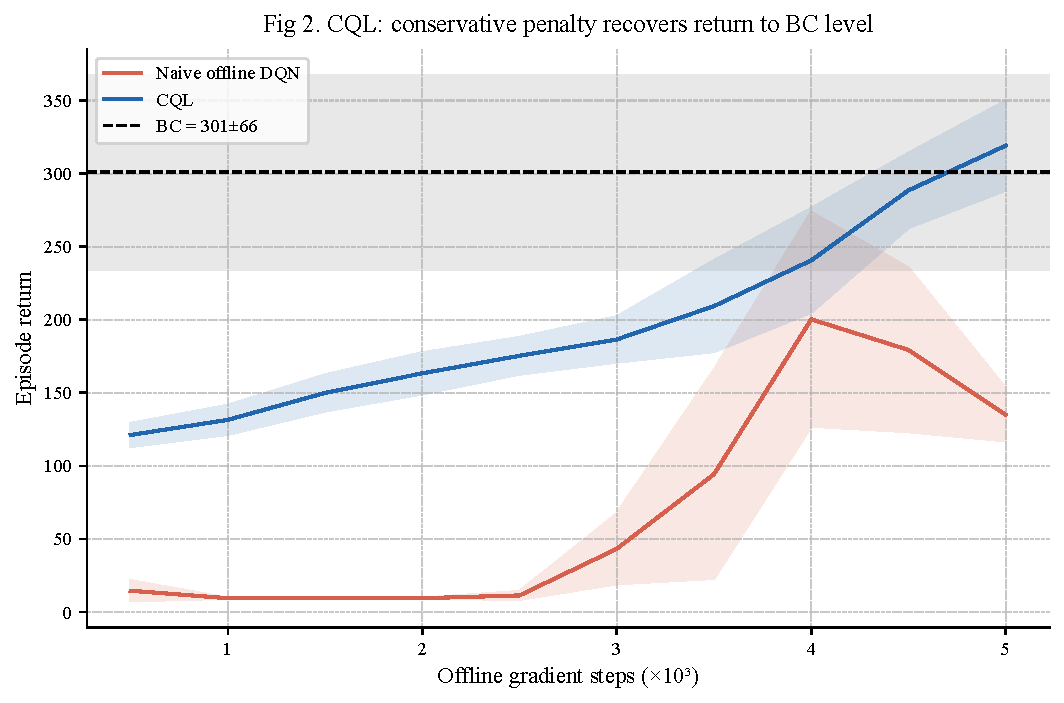
\includegraphics[width=0.88\textwidth]{fig2_cql_conservatism.pdf}
  \caption{CQL's conservative penalty restores returns (CartPole-v1, medium dataset, 3 random seeds, shading $\pm 1\sigma$; the gray band is BC's mean $\pm 1\sigma$). In contrast with the naive offline DQN collapse (red), CQL's return (blue) climbs steadily into the BC band --- no collapse. Same framework, one extra $\alpha\mathcal{R}(s)$ regularizer, from collapse to recovery: the penalty anchors Q onto data-supported actions.}
  \label{fig:cql-conservatism}
\end{figure}

% ============================================================
\section*{Prescription 2: IQL --- writing pessimism into the action set}

\subsection*{Intuition}

Implicit Q-Learning takes the opposite road: \textbf{never evaluate out-of-data actions}. It fits the value function with a special regression target that lets $V$ ``skip'' $\max$ --- since $\max$ is precisely the entry point of out-of-data error.

\subsection*{Expectile regression}

Ordinary least squares fits the conditional \textbf{mean}; IQL uses expectile regression, with a hyperparameter $\tau\in(0,1)$ selecting which quantile of the conditional distribution to fit:

\[
\boxed{L_2^\tau(u) = \bigl|\tau - \mathbf{1}\{u<0\}\bigr|\,u^2}
\]

\begin{itemize}
  \item $\tau = 0.5$ degenerates to ordinary least squares (fitting the mean);
  \item $\tau > 0.5$ (typically $0.7 \sim 0.9$) biases toward \textbf{upper quantiles} --- admitting only ``the better outcomes within the data''.
\end{itemize}

\textbf{In plain words}: online Q-learning answers ``how good could the next step possibly be'' with $\max_{a'} Q(s',\cdot)$; IQL answers the same question by expectile but \textbf{only from $(s',a')$ pairs that truly occurred in the data}. The answer keeps optimism about good actions while never reaching outside the data for a value.

\subsection*{Value and policy updates}

$V$ and $Q$ regress alternately:

\[
\boxed{V_\psi(s) \;\leftarrow\; \arg\min_V \mathbb{E}_{(s,a)\sim\mathcal{D}}\!\left[L_2^\tau\!\bigl(Q_{\bar\theta}(s,a) - V_\psi(s)\bigr)\right]}
\]

\[
\boxed{Q_\theta(s,a) \;\leftarrow\; \arg\min_Q \mathbb{E}_{(s,a,s')\sim\mathcal{D}}\!\left[\bigl(Q_\theta(s,a) - r - \gamma V_\psi(s')\bigr)^2\right]}
\]

\begin{itemize}
  \item $V$ regresses only from in-data actions' $Q_{\bar\theta}$; $\tau$ decides whether it leans toward good actions or the mean;
  \item $Q$'s target contains \textbf{no $\max$}, only $r + \gamma V(s')$ --- extrapolation error has no entry point.
\end{itemize}

The policy updates by AWR-style weighted supervised learning, boosting only actions ``whose in-data value exceeds $V$'':

\[
\boxed{\pi_\phi \;\leftarrow\; \arg\max_\pi \mathbb{E}_{(s,a)\sim\mathcal{D}}\!\left[\exp\!\Big(\frac{1}{\lambda}\bigl(Q_\theta(s,a) - V_\psi(s)\bigr)\Big)\log\pi_\phi(a|s)\right]}
\]

where $\lambda>0$ is the \textbf{temperature} trading off behavior cloning against value improvement: as $\lambda\to\infty$ the weights tend to $1$, degenerating to pure BC; as $\lambda\to 0$ the weights concentrate on the highest-advantage actions, degenerating to greedy Q maximization.

\begin{figure}[!htbp]
  \centering
  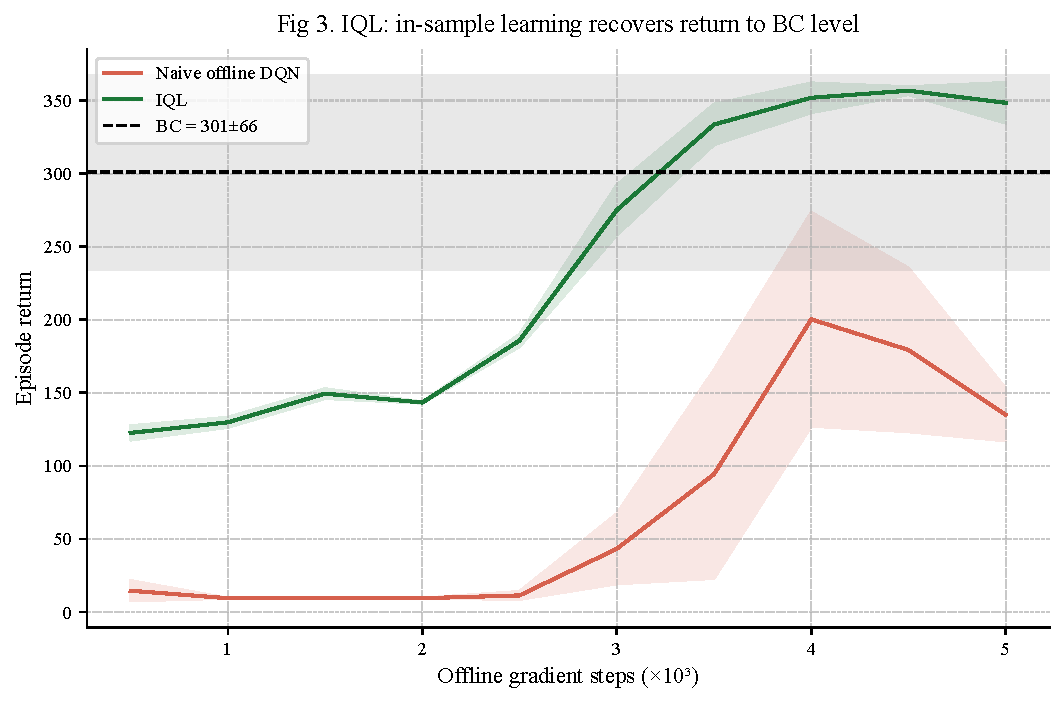
\includegraphics[width=0.88\textwidth]{fig3_iql_insample.pdf}
  \caption{IQL's in-sample learning restores returns (CartPole-v1, medium dataset, 3 random seeds, shading $\pm 1\sigma$; the gray band is BC's mean $\pm 1\sigma$). In contrast with the naive offline DQN collapse (red), IQL's return (green) climbs steadily into the BC band --- no collapse. It never queries out-of-data actions, so extrapolation error never enters the bootstrap target. One disease, a different ``don't ask'' medicine, equally effective.}
  \label{fig:iql-insample}
\end{figure}

% ============================================================
\section*{Two kinds of pessimism: CQL vs IQL}

\subsection*{One disease, two medicines}

\begin{center}
\begin{tabular}{c|c|c}
 & \textbf{CQL} & \textbf{IQL} \\
\hline
Object of pessimism & the value function (pushes OOD Q down) & the action set (never evaluates OOD) \\
Queries out-of-data actions? & yes, but devalues them & never \\
Bootstrap target & penalized $\max$ & $r + \gamma V$ (no $\max$) \\
Key hyperparameters & conservatism $\alpha$ & expectile $\tau$, temperature $\lambda$ \\
Core operator & $\log\sum_a\exp Q$ & expectile regression $L_2^\tau$ \\
\end{tabular}
\end{center}

\textbf{The philosophical difference}: CQL answers ``\underline{how much are out-of-data actions worth}'' --- it forces an answer, but a negative (conservative) one; IQL answers ``\underline{don't answer out-of-data questions}'' --- it changes the question itself, removing $\max$ from the algorithm. The first sets a penalty for liars; the second simply does not ask those who cannot know.

\textbf{In practice}: IQL's AWR-style policy extraction tends to fit the ``offline training $+$ online fine-tuning'' workflow better; fine-tuning CQL online requires explicitly annealing the conservatism $\alpha$ --- the penalty does not vanish on its own, and excessive conservatism blocks further improvement. IQL is also simpler and equally natural for discrete and continuous actions --- it needs no estimate of the behavior policy's action density (in the continuous case CQL must sample extra $a\sim\hat\mu$), only the data's own $(s,a)$ pairs. Each excels on the D4RL benchmarks, but both restore returns stably to the BC pass line --- the message of Figures~2 and 3: two roads to the same destination.

% ============================================================
\section*{Where this chapter sits in the RL landscape}

\begin{enumerate}
  \item \textbf{The value route} $\to$ DQN (online $\max$) $\to$ double Q / target networks (mitigating overestimation);
  \item \textbf{The off-policy route} $\to$ \underline{SAC} (previous chapter: replay reuse) --- offline RL is ``unplugging the environment and freezing the buffer into the whole dataset'';
  \item \underline{Offline RL} (this chapter: no interaction, read-only fixed data $\to$ distribution shift $\to$ CQL devalues OOD / IQL never asks about OOD);
  \item \textbf{Downstream} $\to$ extensions of conservatism (model-based offline methods); the Decision Transformer (Chapter 11) answers the same question with a sequence-modeling worldview.
\end{enumerate}

Offline RL is a key step toward industrial deployment: real-system data is expensive and risky; often only historical data exists. The two prescriptions represent the field's two mainstream ``pessimistic'' designs --- constraining values or constraining actions --- jointly establishing the pass-line mindset: not collapsing (restoring BC's level) matters more than being clever (chasing the optimum).

\subsection*{References}

\begin{enumerate}
  \item Kumar et al.\ (2020). Conservative Q-Learning for Offline Reinforcement Learning. \textit{NeurIPS}.
  \item Kostrikov, Nair \& Levine (2021). Offline Reinforcement Learning with Implicit Q-Learning. \textit{NeurIPS}.
  \item Fujimoto, Meger \& Precup (2019). Off-Policy Deep Reinforcement Learning without Exploration. \textit{ICML}.
  \item Levine et al.\ (2020). Offline Reinforcement Learning: Tutorial, Review, and Perspectives on Practical Applications. \textit{arXiv:2005.01643}.
  \item Pomerleau (1991). Efficient Training of Artificial Neural Networks for Autonomous Navigation. \textit{Neural Computation}.
  \item Sutton \& Barto (2018). \textit{Reinforcement Learning: An Introduction} (2nd ed.). Chapter 13.
\end{enumerate}

\end{document}
